% Zero-shot classification on the shared sphere — TikZ source. Compiles to a tight
% standalone PDF (pdflatex figures/zeroshot-sphere.tex), which
% `book-scaffold build-figures` converts to public/figures/zeroshot-sphere.svg.
%
% Class-name text embeddings sit on the unit circle; an image embedding is
% classified as its nearest text embedding (contrastive alignment).
\documentclass[tikz,border=3pt]{standalone}
\usepackage{amsmath}
\usepackage{amssymb}
\usepackage{tikz}
\usetikzlibrary{positioning,arrows.meta,calc}
\begin{document}
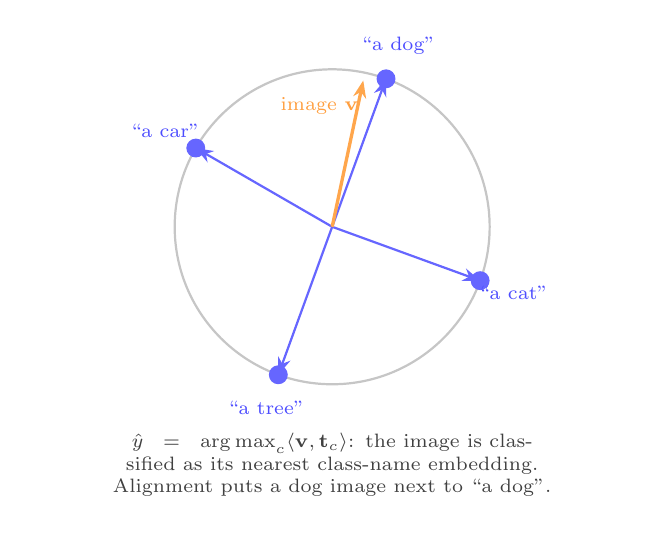
\begin{tikzpicture}[
    font=\small,
    txtv/.style={->, >={Stealth[length=2.2mm]}, blue!60, thick},
    imgv/.style={->, >={Stealth[length=2.2mm]}, orange!70, very thick},
    dot/.style={circle, fill=blue!60, inner sep=0pt, minimum size=2.4mm},
  ]
  \draw[gray!45, thick] (0,0) circle (2);
  % class-name text embeddings on the circle
  \foreach \a/\lbl in {70/{``a dog''}, 150/{``a car''}, 250/{``a tree''}, 340/{``a cat''}} {
    \draw[txtv] (0,0) -- (\a:2);
    \node[dot] at (\a:2) {};
    \node[font=\scriptsize, text=blue!70] at (\a:2.45) {\lbl};
  }
  % image embedding near "a dog"
  \draw[imgv] (0,0) -- (78:1.9);
  \node[font=\scriptsize, text=orange!75] at (96:1.55) {image $\mathbf v$};

  \node[below, align=center, text width=7.5cm, font=\scriptsize, text=black!75]
    at (0,-2.5)
    {$\hat y=\operatorname*{arg\,max}_c\langle\mathbf v,\mathbf t_c\rangle$: the image is classified as its
     nearest class-name embedding. Alignment puts a dog image next to ``a dog''.};
\end{tikzpicture}
\end{document}
